% Auriga theme
% https://github.com/anishathalye/auriga

\documentclass[14pt,aspectratio=169]{beamer}
\usepackage{pgfpages}
\usepackage{fancyvrb}
\usepackage{booktabs,dcolumn}
\usepackage{tikz}
\usetikzlibrary{arrows.meta, positioning, quotes}
\usepackage{pgfplots}

% \ifnotes
% \setbeamertemplate{note page}[plain]
% \setbeameroption{show notes on second screen=right}
% \fi

\usetheme{auriga}
\usecolortheme{auriga}

% define some colors for a consistent theme across slides
\definecolor{red}{RGB}{181, 23, 0}
\definecolor{blue}{RGB}{0, 118, 186}
\definecolor{gray}{RGB}{146, 146, 146}

\title{Historia Económica Argentina}

\author{\underline{Sebastián Freille} \inst{1}}

\institute[shortinst]{\inst{1} IEF-UNC \\ UCC}
\date{}

\AtBeginSection[]{
    \begin{frame}
    \vfill
    \centering
    \begin{beamercolorbox}[sep=8pt,center,shadow=true,rounded=true]{title}
        \usebeamerfont{title}\insertsectionhead\par%
    \end{beamercolorbox}
    \vfill
    \end{frame}
}



\AtBeginSubsection[]{
    \begin{frame}
    \vfill
    \centering
    \begin{beamercolorbox}[sep=6pt,center,shadow=true,rounded=true]{title}
        \usebeamerfont{title}\insertsubsectionhead\par%
    \end{beamercolorbox}
    \vfill
    \end{frame}
}


\AtBeginSubsubsection[]{
    \begin{frame}
    \vfill
    \centering
    \begin{beamercolorbox}[sep=4pt,center,shadow=true,rounded=true]{title}
        \usebeamerfont{title}\insertsubsubsectionhead\par%
    \end{beamercolorbox}
    \vfill
    \end{frame}
}


\begin{document}

{
  % rather than use the frame options [noframenumbering,plain], we make the
  % color match, so that the indicated page numbers match PDF page numbers
  \setbeamercolor{page number in head/foot}{fg=background canvas.bg}
  \begin{frame}
    \titlepage
  \end{frame}
}

  
  \section{Capítulo 4. Liberalización de los mercados en el período 1955-1963}


  \section{Contexto}
  

 \begin{frame}\frametitle{Clima político enrarecido}
    \begin{itemize}\itemsep 10pt
      \item Ya desde el año 1949 (Convención Constituyente), el clima
        político estaba enrarecido --varios partidos decidieron no
        participar y la UCR se retiró.
        \item Esto coincidió con un endurecimiento del discurso de
          Perón y una gradual intolerancia hacia sus críticos y
          opositores --persecución y ataques a opositores
          \item Medios de comunicación adquiridos por el gobierno y
            otros clausurados y expropiados --esto pasaba en diarios y
            radio. 
                        \end{itemize}
               \end{frame}


               
 \begin{frame}\frametitle{Clima político enrarecido (cont.)}
    \begin{itemize}\itemsep 10pt
      \item El radicalismo tenía lineas internas --unionistas e
        intransigentes. Los primeros proponían linea dura
        (``abstencionismo y revolución''), los segundos la lucha
        democrática y parlamentaria
        \item A pesar del avasallador triunfo de Perón en 1952, la
          minoría política antiperonista profundizó su resistencia y
          su lucha a la espera de una ocasión propicia
          \item Paradoja $\longrightarrow$ mientras economía se
            recuperaba en 1952-55, había cada mayores tensiones políticas
                 \end{itemize}
               \end{frame}


 \begin{frame}\frametitle{Clima político enrarecido (cont.)}
    \begin{itemize}\itemsep 10pt
      \item Aún así, no era extraña la idea de que Perón concluyera su
        segundo mandato $\longrightarrow$ oposición debilitada
        electoralmente y sin acceso a medios
        \item Militares muy debilitados luego de la purga en 1951
          detrás del fallido golpe
          \item Un inesperado giro en la relación entre Perón y la
            Iglesia escaló en un conflicto de proporciones
            $\longrightarrow$ oposición vio una oportunidad de
            capturar el poder
                             \end{itemize}
               \end{frame}

               \begin{frame}\frametitle{Clima político enrarecido (cont.)}
    \begin{itemize}\itemsep 10pt
      \item El año 1955 vería tres sucesos centrales en el cambio de
        la dinámica política y económica:
        \begin{itemize}\itemsep 5pt \medskip
        \item Bombardeo de plaza de Mayo (16 de junio de 1955)
          \item Toma de la Escuela de Artillería de Córdoba por parte
            de Lonardi (16 de
            septiembre)
            \item Renuncia sin resistencia y huída de Perón
          \end{itemize}
          \item Es relevante mencionar que gran parte del éxito del
            golpe cívico-militar se debió a la posición combativa de
            la Marina (el Ejército, en su mayoría, apoyó a Perón). 
                             \end{itemize}
               \end{frame}


\section{La Revolución Libertadora}
               

                       \begin{frame}\frametitle{La Revolución Libertadora}
                         \begin{block}{``Ni vencedores ni vencidos''}
                          La auto-denominada ``revolución
                          libertadora'' tenía algunos objetivos más
                          claros que las anteriores en que sólo se
                          buscó derrocar al Presidente de turno. La
                          famosa frase del nuevo Presidente de facto,
                          Eduardo Lonardi, ``ni vencedores ni
                          vencidos'' aspiraba a una transición moderada
                          hacia un
                          nuevo orden democrático que pronto quedaría
                          sólo como expresión de deseo. Esta línea
                          blanda de Lonardi pronto daría paso a una
                          línea dura del general Pedro Aramburu.  
                          \end{block}  
               \end{frame}


               \begin{frame}\frametitle{La Revolución Libertadora (cont.)}
                 \begin{itemize}\itemsep 5pt \medskip
                 \item La principal justificación histórica de la
                   Revolución Libertadora fue la de reestablecer la
                   política democrática y un
                   conjunto de instituciones políticas que la
                   promovieran
                   \item En retrospectiva, la ``Libertadora'' no
                     cumplió las expectativas creadas por varias
                     razones. Primero, la posición conciliadora de
                     Lonardi requería consistencia ideológica y de
                     propósito que no tenía. Segundo, la instalación
                     de un régimen de persecución, intolerancia y
                     violencia dirigido al peronismo. 
                   \end{itemize}
               \end{frame}
               

  \begin{frame}\frametitle{La Revolución Libertadora (cont.)}
                 \begin{itemize}\itemsep 5pt \medskip
                 \item Hubo tres razones principales para que la
                   transición de la Revolución Libertadora no fuera ni
                   tan profunda ni tan revolucionaria.
                   \begin{itemize}\itemsep 5pt \medskip
                   \item la situación heredada (``la herencia'') no
                     era tan pesada como aparecía en el discurso
                     \item el nuevo gobierno siempre se pensó como
                       provisorio y no permanente
                       \item varias de lsa políticas más ambiciosas no
                         dieron los frutos esperados
                       \end{itemize}
                       \item En gran parte, la Revolución Libertadora
                         no avanzó en grandes cambios significativos
                         que eran posibles de realizar en función del contexto
                   \end{itemize}
               \end{frame}


 \begin{frame}\frametitle{La política económica de la RL}
                 \begin{itemize}\itemsep 5pt \medskip
                 \item La principal premisa económica de las nuevas
                   autoridades era aumentar las exportaciones y
                   estimular la formación de capital
                   \item Hubo evidentes intentos de modificar los
                     precios relativos $\longrightarrow$ principal
                     cambio la política de devaluación desde 1955
                     \item En 1956, los tipos de cambio de X y M se
                       aumentaron un 100 y un 75 por ciento en
                       términos reales
                       \item La respuesta del sector agropecuario fue
                         moderada --aumento de area sembrada (1956-57) sólo un
                         3.5\% mas que en 1952-54
                   \end{itemize}
               \end{frame}
               

              

 
  \begin{frame}\frametitle{La política económica de la RL (cont.)}
\begin{figure}[hxtbp]\vspace{0cm}
  \centering
  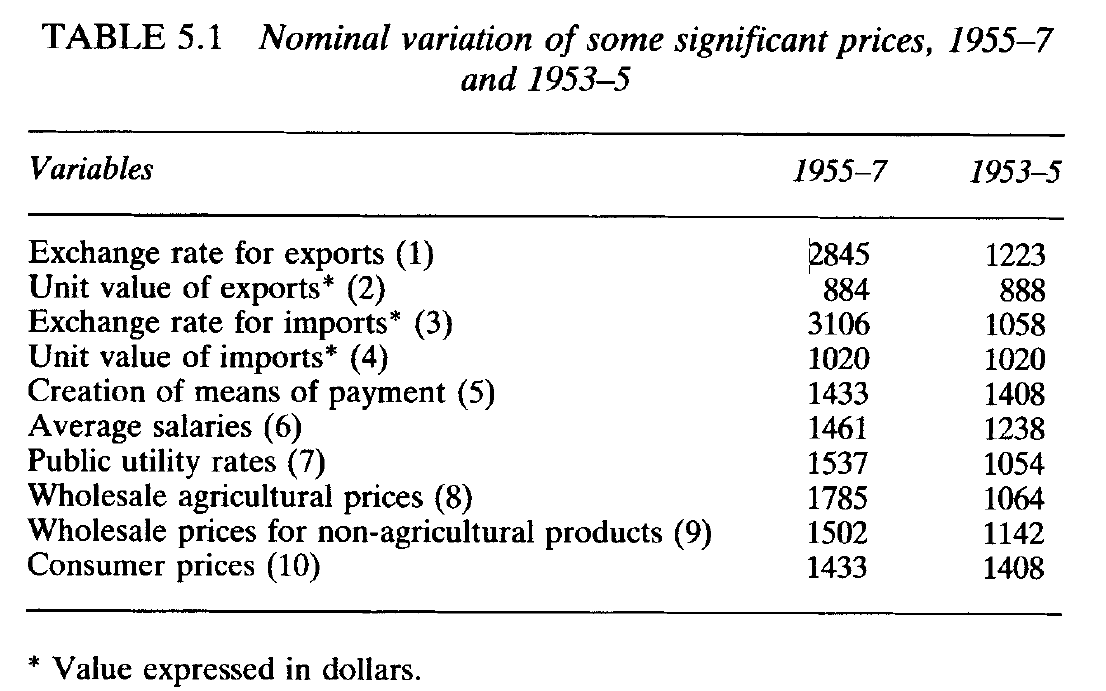
\includegraphics[scale=0.65]{uni4_rl01}
   \label{fig:uni1_01}
\end{figure} 
  \end{frame}
               

                \begin{frame}\frametitle{La política económica de la
                    RL (cont.)}
                 \begin{itemize}\itemsep 5pt \medskip
                 \item Paradójicamente (como luego pasaría en otros
                   momentos de la historia), la economía argentina se
                   estaba abriendo cuando los TIE estaban cayendo
                   fuertemente --en 1957, los TIE eran 44\% menores
                   que en 1948, y 13\% menores que en 1955.
                   \item Por esta razón, hubo balances de pagos
                     negativos en todo el período 1955-58
                     $\longrightarrow$ salida de reservas y crecientes
                     déficits comerciales
                   \item La economía argentina sufría nuevamente en el
                     frente externo
                   \end{itemize}
               \end{frame}



                \begin{frame}\frametitle{La política económica de la
                    RL (cont.)}
                 \begin{itemize}\itemsep 5pt \medskip
                 \item Las autoridades pronto se dieron cuenta de que
                   la única forma de proteger a la industria era la
                   sustitución de M en areas intensivas en tecnología
                   y capital.
                   \item Pero además, el estancamiento de la industria
                     también afectaba al acumulación de capital (un
                     objetivo de la RL) $\longrightarrow$ a pesar de
                     liberar el mercado de cambios mantuvieron
                     permisos anticipados de M hasta 1959 (en que
                     fueron eliminados)
                   \end{itemize}
               \end{frame}
      

  \begin{frame}\frametitle{La política económica de la
                    RL (cont.)}
                 \begin{itemize}\itemsep 5pt \medskip
                 \item Tampoco hubo crédito flexible ni tipo de cambio
                   diferenciales para la acumulación de K
                   $\longrightarrow$ de hecho tasa de inversión cayó
                   levemente en 1955-58
                   \item La inversión pública también se mantuvo baja
                     para no afectar los déficits fiscales
                     \item En muchos aspectos, no fue sino hasta 1960
                       en que se produjeron cambios radicales
                   \end{itemize}
               \end{frame}
               


  \begin{frame}\frametitle{La política económica de la
                    RL (cont.)}
                 \begin{itemize}\itemsep 5pt \medskip
                 \item No se produjeron cambios en los salarios reales
                   $\longrightarrow$ atacaron el poder sindical pero
                   no a costa del estandar de vida de los trabajadores
                   \item En resumidas cuentas, el gobierno militar
                    se resistía a empeorar las condiciones económicas
                    de la gran masa de trabajadores
                    \item Incluso cuando aumentaron precios relativos
                      de productos agropecuarios, usaron subsidios al
                      consumo y controles de precios para evitar un
                      deterioro del salario real
                   \end{itemize}
               \end{frame}


  \begin{frame}\frametitle{La política económica de la
                    RL (cont.)}
                 \begin{itemize}\itemsep 5pt \medskip
                 \item En cierto modo, las autoridades de la RL usaron
                   la discrecionalidad en la política económica cada
                   vez que lo consideraron necesario para no empeorar
                   el clima y las tensiones económicas y sociales (se
                   alejaron de las políticas conservadores que proponían!)
                   \item La RL trajo consigo \textbf{cambios políticos
                       muy significativos y duraderos} pero
                     \textbf{cambios económicos moderados y graduales}
                   \end{itemize}
               \end{frame}


\end{document}





      